\documentclass[tikz,border=12pt]{standalone}
\usepackage[T1]{fontenc}
\usepackage{tikz}
\usetikzlibrary{positioning,arrows.meta,fit,backgrounds,calc}

\definecolor{fglight}{HTML}{e5e5e5}
\definecolor{accent}{HTML}{60a5fa}
\definecolor{muted}{HTML}{999999}
\definecolor{composecolor}{HTML}{f472b6}
\definecolor{templatecolor}{HTML}{a78bfa}
\definecolor{staticcolor}{HTML}{34d399}
\definecolor{boxbg}{HTML}{2a2a2a}

\begin{document}
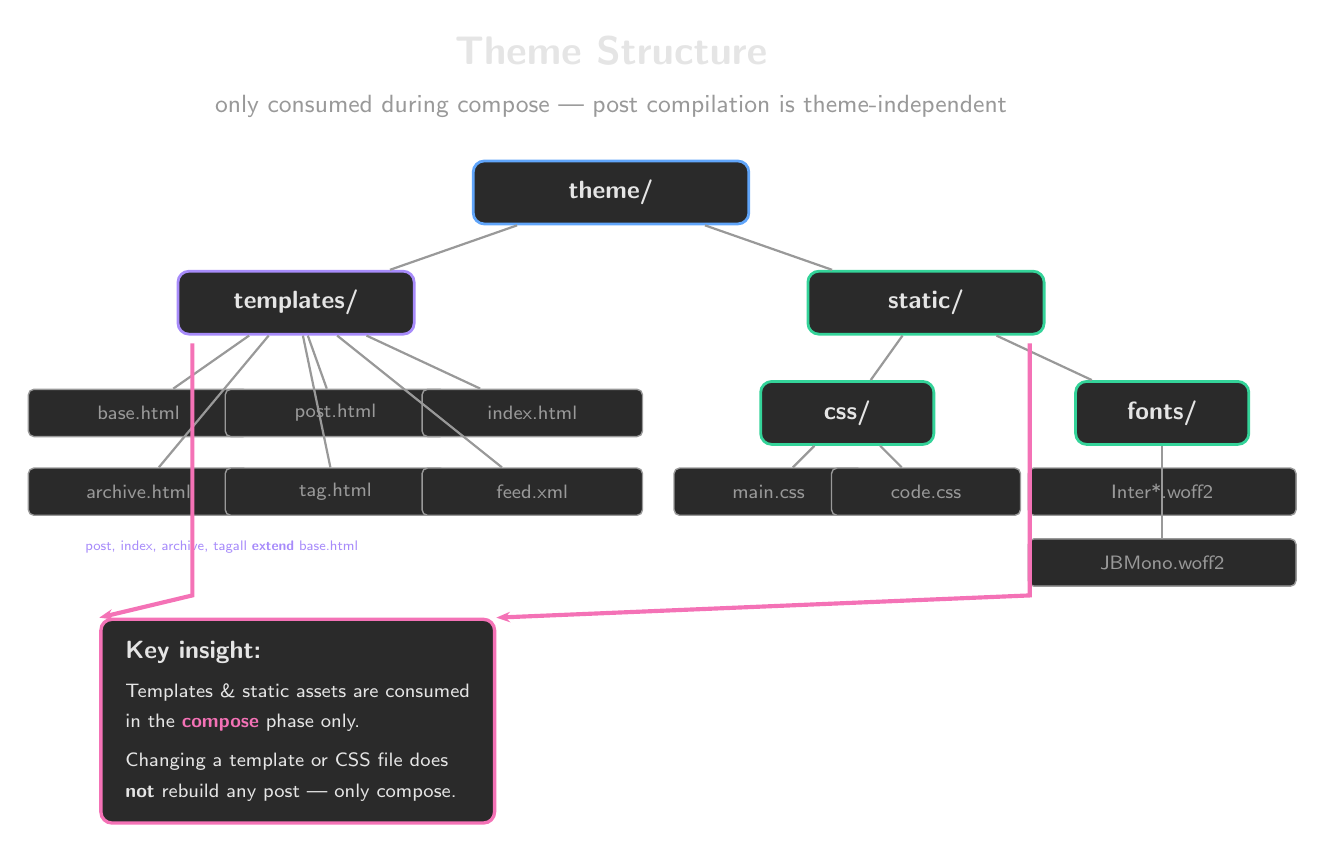
\begin{tikzpicture}[
    >={Stealth[length=5pt]},
    every node/.style={font=\sffamily},
    dirnode/.style={
        rounded corners=4pt,
        minimum height=0.8cm,
        align=center,
        text=fglight,
        draw=#1,
        line width=1pt,
        fill=boxbg,
        font=\sffamily\small,
    },
    filenode/.style={
        rounded corners=2pt,
        minimum width=2.8cm,
        minimum height=0.6cm,
        align=center,
        text=muted,
        draw=muted,
        line width=0.5pt,
        fill=boxbg,
        font=\sffamily\scriptsize,
    },
    connector/.style={-,line width=0.8pt,color=muted},
    note/.style={font=\sffamily\scriptsize,text=muted,align=left},
]

% === Title ===
\node[font=\sffamily\Large\bfseries,text=fglight] at (0,8) {Theme Structure};
\node[font=\sffamily\small,text=muted] at (0,7.3) {only consumed during compose --- post compilation is theme-independent};

% === Root ===
\node[dirnode=accent,minimum width=3.5cm] (root) at (0,6.2) {\textbf{theme/}};

% === Two branches ===
\node[dirnode=templatecolor,minimum width=3cm] (templates) at (-4,4.8) {\textbf{templates/}};
\node[dirnode=staticcolor,minimum width=3cm] (static) at (4,4.8) {\textbf{static/}};

\draw[connector] (root) -- (templates);
\draw[connector] (root) -- (static);

% === Template files (2 rows, well spaced) ===
\node[filenode] (base) at (-6,3.4) {base.html};
\node[filenode] (post) at (-3.5,3.4) {post.html};
\node[filenode] (index) at (-1,3.4) {index.html};

\node[filenode] (archive) at (-6,2.4) {archive.html};
\node[filenode] (tag) at (-3.5,2.4) {tag.html};
\node[filenode] (feed) at (-1,2.4) {feed.xml};

\draw[connector] (templates) -- (base);
\draw[connector] (templates) -- (post);
\draw[connector] (templates) -- (index);
\draw[connector] (templates) -- (archive);
\draw[connector] (templates) -- (tag);
\draw[connector] (templates) -- (feed);

% === Template inheritance note (simple, no arrows) ===
\node[font=\sffamily\tiny,text=templatecolor,anchor=west] at (-6.8,1.7) {
    post, index, archive, tag\\
    all \textbf{extend} base.html
};

% === Static files ===
\node[dirnode=staticcolor,minimum width=2.2cm] (css) at (3,3.4) {\textbf{css/}};
\node[dirnode=staticcolor,minimum width=2.2cm] (fonts) at (7,3.4) {\textbf{fonts/}};

\draw[connector] (static) -- (css);
\draw[connector] (static) -- (fonts);

\node[filenode,minimum width=2.4cm] (maincss) at (2,2.4) {main.css};
\node[filenode,minimum width=2.4cm] (codecss) at (4,2.4) {code.css};

\node[filenode,minimum width=3.4cm] (inter) at (7,2.4) {Inter*.woff2};
\node[filenode,minimum width=3.4cm] (jbm) at (7,1.5) {JBMono.woff2};

\draw[connector] (css) -- (maincss);
\draw[connector] (css) -- (codecss);
\draw[connector] (fonts) -- (inter);
\draw[connector] (fonts) -- (jbm);

% === Key insight box ===
\node[
    rounded corners=4pt,
    draw=composecolor,
    line width=1.2pt,
    fill=boxbg,
    text=fglight,
    font=\sffamily\small,
    align=left,
    minimum width=5cm,
    inner sep=8pt,
    anchor=north west,
] (insight) at (-6.5,0.8) {
    \textbf{Key insight:}\\[3pt]
    {\scriptsize Templates \& static assets are consumed}\\
    {\scriptsize in the \textcolor{composecolor}{\textbf{compose}} phase only.}\\[3pt]
    {\scriptsize Changing a template or CSS file does}\\
    {\scriptsize \textbf{not} rebuild any post --- only compose.}
};

% === Compose arrow ===
\draw[->,line width=1.5pt,color=composecolor]
    (templates.south west) ++(0.2,-0.1) -- ++(0,-3.2) -- (insight.north west);
\draw[->,line width=1.5pt,color=composecolor]
    (static.south east) ++(-0.2,-0.1) -- ++(0,-3.2) -- (insight.north east);

\end{tikzpicture}
\end{document}
